\section{Implementation}
\label{sec:implementation}

In our implementation, we confine ourselves to analyzing JavaScript projects for node.js.
This decision is based on the large prevalence of JavaScript\footnote{GitHut 2.0: A small place to discover languages in GitHub. \url{https://madnight.github.io/githut/\#/pushes}} as well as the first-rate extent of the npm ecosystem which has been unsurpassed since 2015\footnote{Modulecounts: \url{http://www.modulecounts.com/}}.
In the following, we describe how we apply the single steps of the approach presented above to this domain.

\subsection{Downstream Dependency Collection}
\label{sec:implementation/dependency_collection}

The de facto standard package repository for node.js is npm.
To fetch downstream dependency packages from the npm registry, we use the npm package \code{npm-dependants}\footnote{All packages can be retrieved from \url{npmjs.com}} which scrapes the dependents list from npmjs.com as there does not exist a publicly available API for these data.
To keep the footprint of our implementation small, we only scrape a part of the dependents list.
We then request basic metadata for each found package from the npm registry, including the \emph{tarball} URL of the latest package version, using the package \code{package-metadata}.
Finally, we download and extract each tarball using the package \code{download-package-tarball}.

\begin{lstlisting}[language=json,
	label=sec:implementation/package.json,
	caption={An example \code{package.json} file for the \code{ripple-lib} package specifying multiple dependencies (truncated).},
	float=tpb,
	floatplacement=tbp,
	abovecaptionskip=-5pt
]
{
	"name": "ripple-lib",
	"version": "1.10.0",
	"description": "An API for the XRP Ledger",
	"dependencies": {
		"bignumber.js": "^9.0.0",
		"https-proxy-agent": "^5.0.0",
		"jsonschema": "1.2.2"
	}
}
\end{lstlisting}

For the second approach based on a code search engine, we have identified Sourcegraph\footnote{\url{https://sourcegraph.com/}} as a promising platform.
npm packages specify their dependencies in a package.json metadata file (see \cref{sec:implementation/package.json}).
To find all packages depending on a certain package, we can search all available \code{package.json} files for a reference to this package identifier.
We refine our search query with some additional constraints to filter out package copies from \code{node_modules} folders that downstream developers have pushed accidentally, and to limit the number of results retrieved.
We submit this search query to the publicly available GraphQL\footnote{\url{https://graphql.com/}} API of Sourcegraph\footnote{\url{https://docs.sourcegraph.com/api/graphql}} by using the npm package \code{graphql-request}.
After retrieving a search result, we download a snapshot of the full repository by using the package \code{download-git-repo}.

Additionally, we enrich the metadata of each package with a few metrics indicating its popularity from the associated GitHub repository if specified.
The GitHub API is accessed via the official \emph{octokit} library\footnote{\url{https://octokit.github.io/}}.

\subsection{Usage Sample Mining}
\label{sec:implementation/usage_mining}

For parsing the dependencies, we utilize the \emph{TypeScript Compiler API}\footnote{\url{https://github.com/Microsoft/TypeScript/wiki/Using-the-Compiler-API}}.
TypeScript is an extension of JavaScript that adds strong typing to the former; typing is based on a combination of implicit type inference and explicit type declarations.
As the type-checking capabilities of the TypeScript compiler are optional and can be turned off via configuration, we consider the JavaScript syntax a subset of TypeScript syntax.
As a side benefit, our implementation is also able to analyze packages implemented in true TypeScript.

The TypeScript compiler's \emph{binder} component annotates every node of the parsed program with a type symbol if it can resolve one.
After performing a type analysis of the dependency by instrumenting the binder, we collect all nodes from the type-annotated ASF that refer to the target package by traversing it with a visitor function.
This visitor function matches each node against a list of defined patterns (similar to \cref{fig:approach/usage_mining/patterns}) based on the syntax kinds of the node, its ancestors, and its descendants, and then performs a lookup of the node's type symbol's declaration to compare it with the source directory of the target package.

Normally, foreign types can only be resolved if they are declared in a dependency module that has been installed into the \code{node_modules} folder of the repository.
Because downloading and installing all dependency modules for every downstream repository of the target package would increase the computational resources of the usage mining drastically and eventually violate \cref{req1}, we skip this step but instead modify the module resolution strategy of the TypeScript compiler host.
To do so, we extend the \code{paths} parameter from the default compiler options\footnote{\url{https://www.typescriptlang.org/tsconfig\#paths}} and insert a new entry that remaps accesses to the target package name to the separate source code directory of the target package.

\begin{figure*}
	\centering
	\begin{subfigure}{.32\linewidth}
		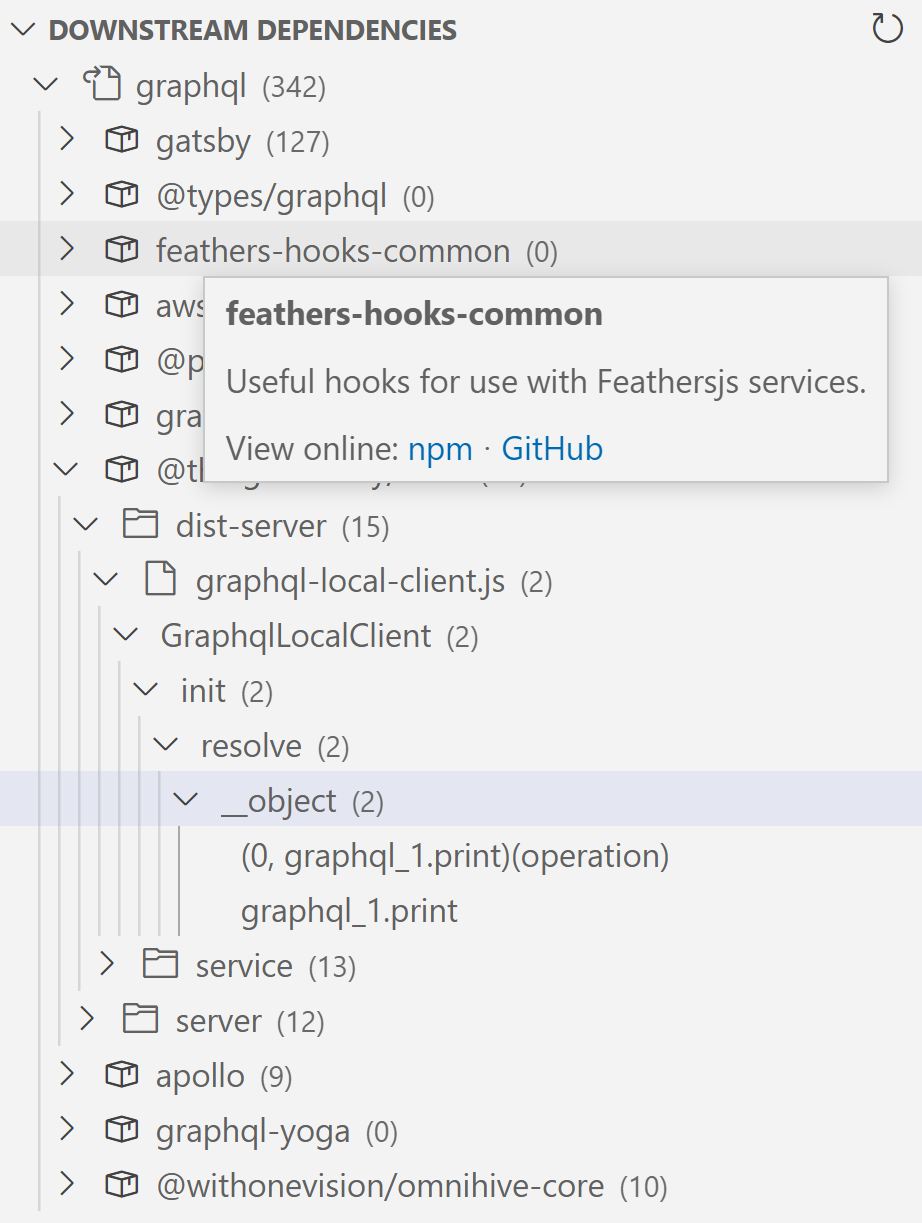
\includegraphics[width=\linewidth]{sections/4_implementation/extension/dependencies.png}
		\caption[LoF entry]{The dependency browser.}
		\label{fig:implementation/presentation/screenshot/dependency_browser}
	\end{subfigure}
	\hfill
	\begin{subfigure}{.32\linewidth}
		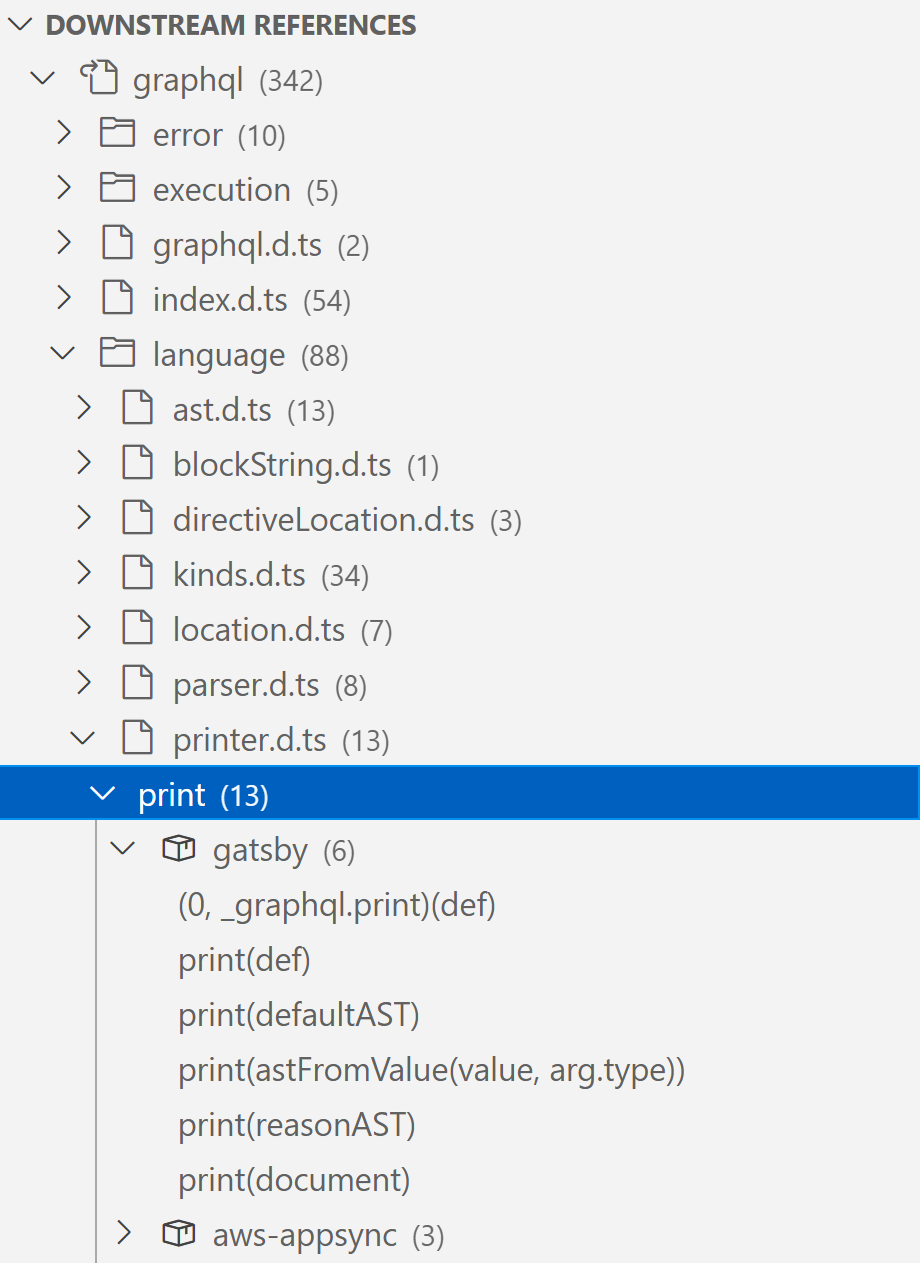
\includegraphics[width=\linewidth]{sections/4_implementation/extension/references.png}
		\caption[LoF entry]{The usage browser.}
		\label{fig:implementation/presentation/screenshot/usage_browser}
	\end{subfigure}
	\hfill
	\begin{subfigure}{.32\linewidth}
		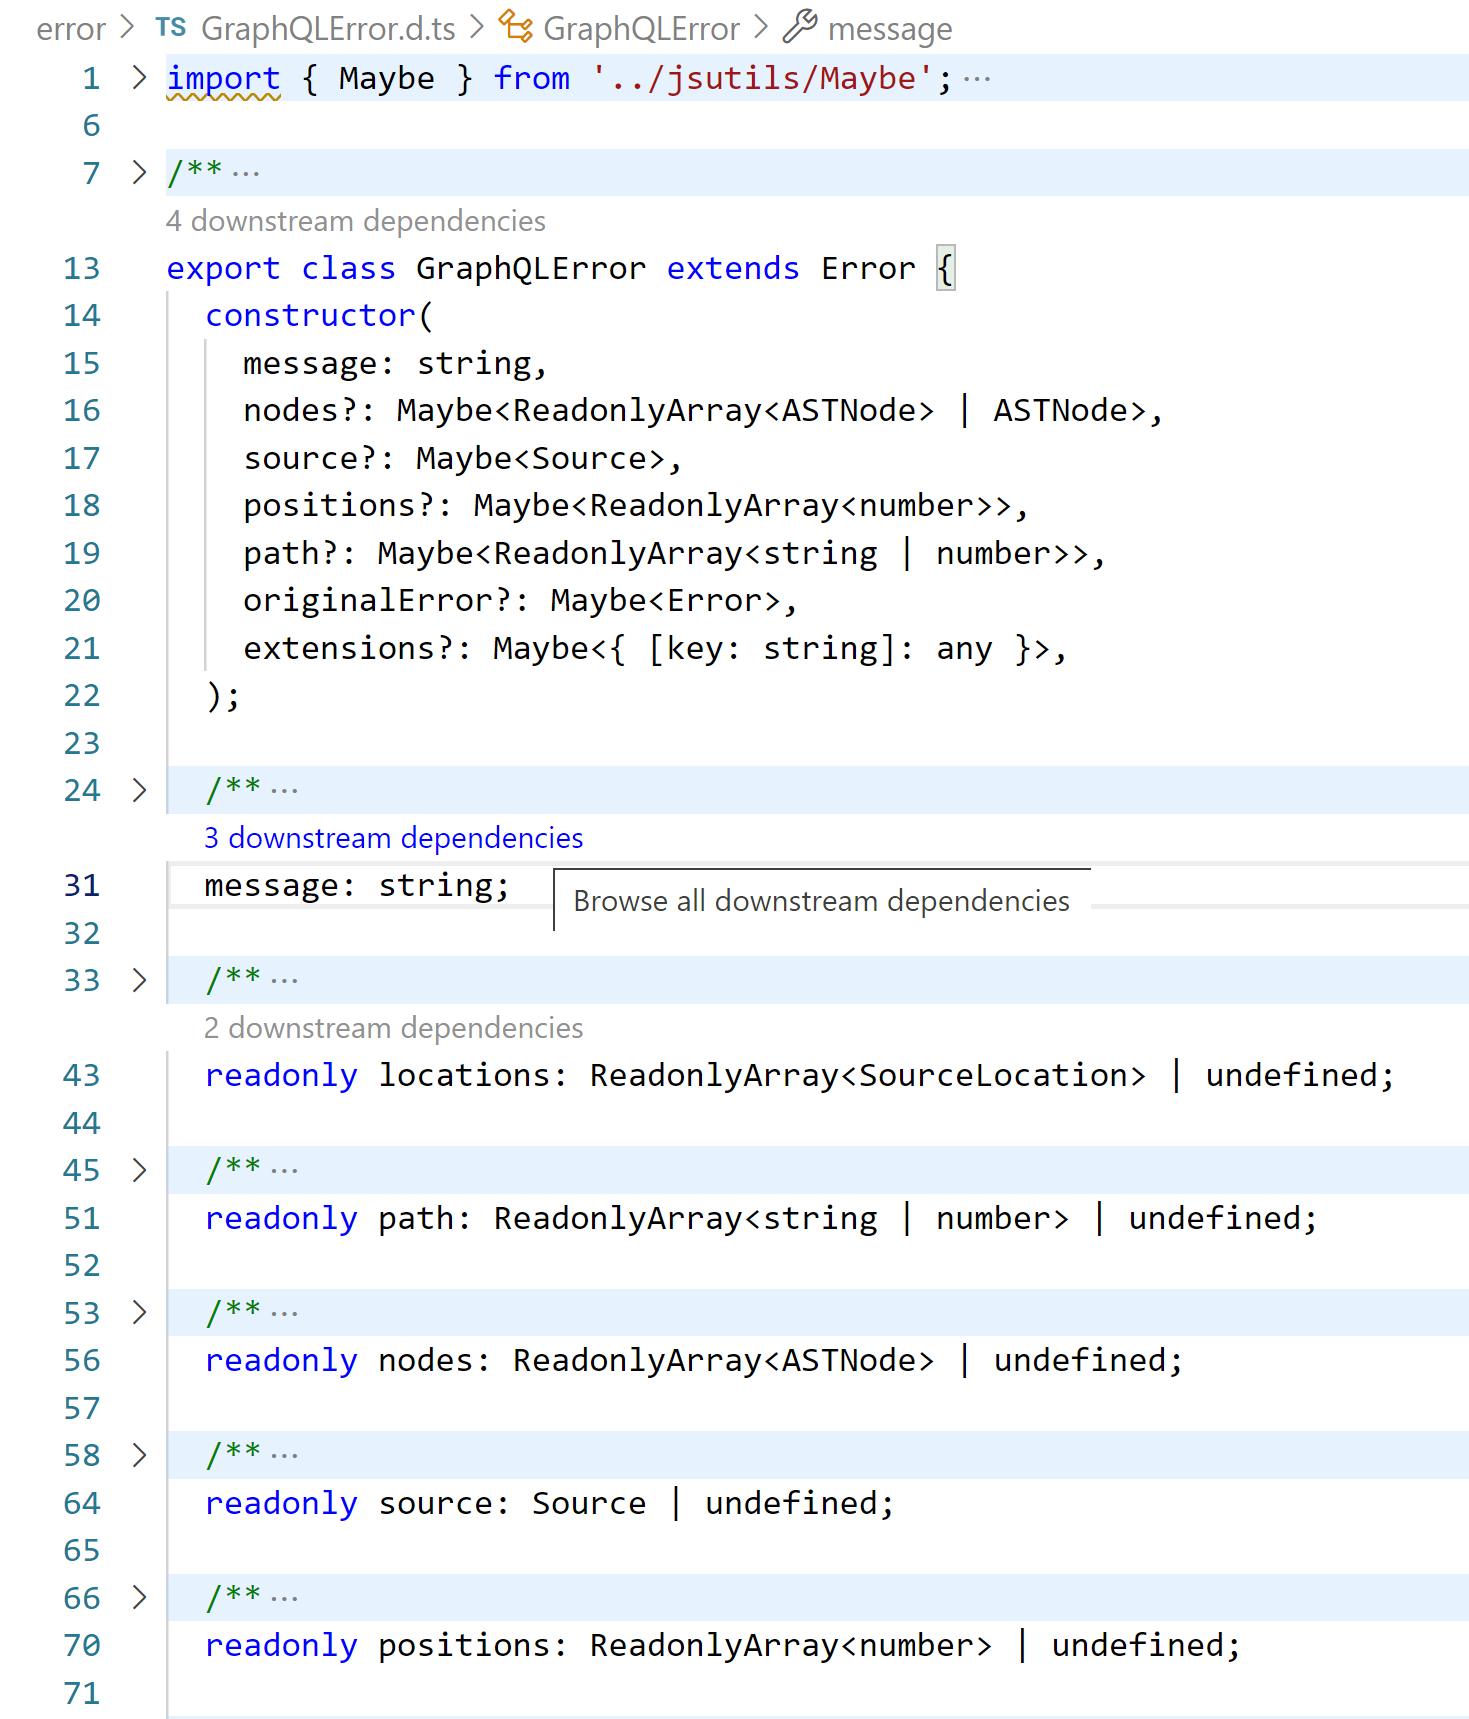
\includegraphics[width=\linewidth]{sections/4_implementation/extension/codelens.png}
		\caption[LoF entry]{The CodeLens integration for the class \code{GraphQLError}.}
		\label{fig:implementation/presentation/screenshot/codelens}
	\end{subfigure}

	\caption{Screenshots of our VS Code extension used to explore downstream dependencies of the npm package graphql.}
	\label{fig:implementation/presentation/screenshots}
\end{figure*}

\subsection{Presentation of Results}
\label{sec:implementation/presentation}

After all references have been collected, a proper UI is still required to provide users easy access to these data that fulfills the requirements mentioned above.
To satisfy \cref{req2} and make our tool available in the usual working environment of users, we implement it as an extension to the \emph{Visual Studio Code} IDE\footnote{\url{https://code.visualstudio.com/}}.
VS Code is one of the most popular IDEs that support JavaScript, and the one with the highest annual growth.\footnote{Top IDE Index by Pierre Carbonnelle (2021): \url{https://pypl.github.io/IDE.html}}
It also provides a comprehensive set of APIs for extension developers.
To support other researchers in reusing our solution, we also provide a CLI.

To support developers in answering the questions raised in \cref{sec:approach}, we have designed three key views for our extension (see \cref{fig:implementation/presentation/screenshots}):

\begin{enumerate}[label=(\roman*)]
	\item The \emph{dependency browser} allows to explore all downstream dependencies and, grouped for each dependency, all their references to the target package.
	\item The \emph{usage browser} displays all public package members and, grouped for each member, all dependencies and their references to this member.
	\item The \emph{CodeLens integration} provides quick access to a slice usage samples and is attached to the definition of each package member in the source code editor.
\end{enumerate}

Both references and members are organized in a tree view reflecting the hierarchical structure of the original software repository.
In addition, we recognize the effort of browsing large lists of dependency data and encounter it by providing an ``I'm feeling lucky'' button for every view that redirects the user to a random dependency or reference, resp., to gain a faster, unbiased impression of usage samples.

We implement each of these views in the VS Code Extension API (VSCE)\footnote{\url{https://code.visualstudio.com/api}}, we use the \emph{Tree View API} and the \emph{CodeLens API}.
One challenge has been to deliver fast results and not to block the user interface because even in spite of the lightweight mining approaches we chose to satisfy \cref{req1} above, querying, downloading, and analyzing each dependency takes a few seconds (see \cref{sec:evaluation}).
To overcome this issue, we use pagination wherever possible and apply the observer pattern to push incremental UI updates.
As the VSCE API per se does not provide for multithreading or multiprocessing operations but suggests a Promise/A+-driven dataflow, we adopt this style for our object model by using the JavaScript concepts asynchronous functions, \code{AsyncIterator}s, and \code{Promise.all} to avoid busy waiting inside the data collection process.
